\subsection{Métricas de Evaluación para Sistemas de Clasificación}

La evaluación cuantitativa del desempeño de sistemas de clasificación requiere métricas que capturen la calidad predictiva del modelo. En aplicaciones de agricultura de precisión, donde decisiones incorrectas pueden impactar la productividad del cultivo, resulta fundamental seleccionar métricas apropiadas que reflejen los objetivos operativos del sistema.

\subsubsection{Matriz de Confusión}

La matriz de confusión constituye la representación fundamental del desempeño de un clasificador, tabulando predicciones versus etiquetas verdaderas. Para un problema de $C$ clases, la matriz de confusión $\mathbf{M} \in \mathbb{R}^{C \times C}$ tiene elementos:

\begin{equation}
M_{ij} = \sum_{k=1}^{N} \mathbb{1}[y_k = i \land \hat{y}_k = j]
\end{equation}

donde $y_k$ es la clase verdadera de la muestra $k$, $\hat{y}_k$ es la clase predicha, y $\mathbb{1}[\cdot]$ es la función indicadora. El elemento $M_{ij}$ cuenta cuántas muestras de la clase $i$ fueron clasificadas como clase $j$. Los elementos diagonales representan clasificaciones correctas, mientras que los elementos fuera de la diagonal representan errores.

Para clasificación binaria, la matriz distingue cuatro categorías: verdaderos positivos (TP), verdaderos negativos (TN), falsos positivos (FP, Error Tipo I), y falsos negativos (FN, Error Tipo II). Esta descomposición permite calcular métricas más específicas que la exactitud global.

\begin{figure}[h]
\centering
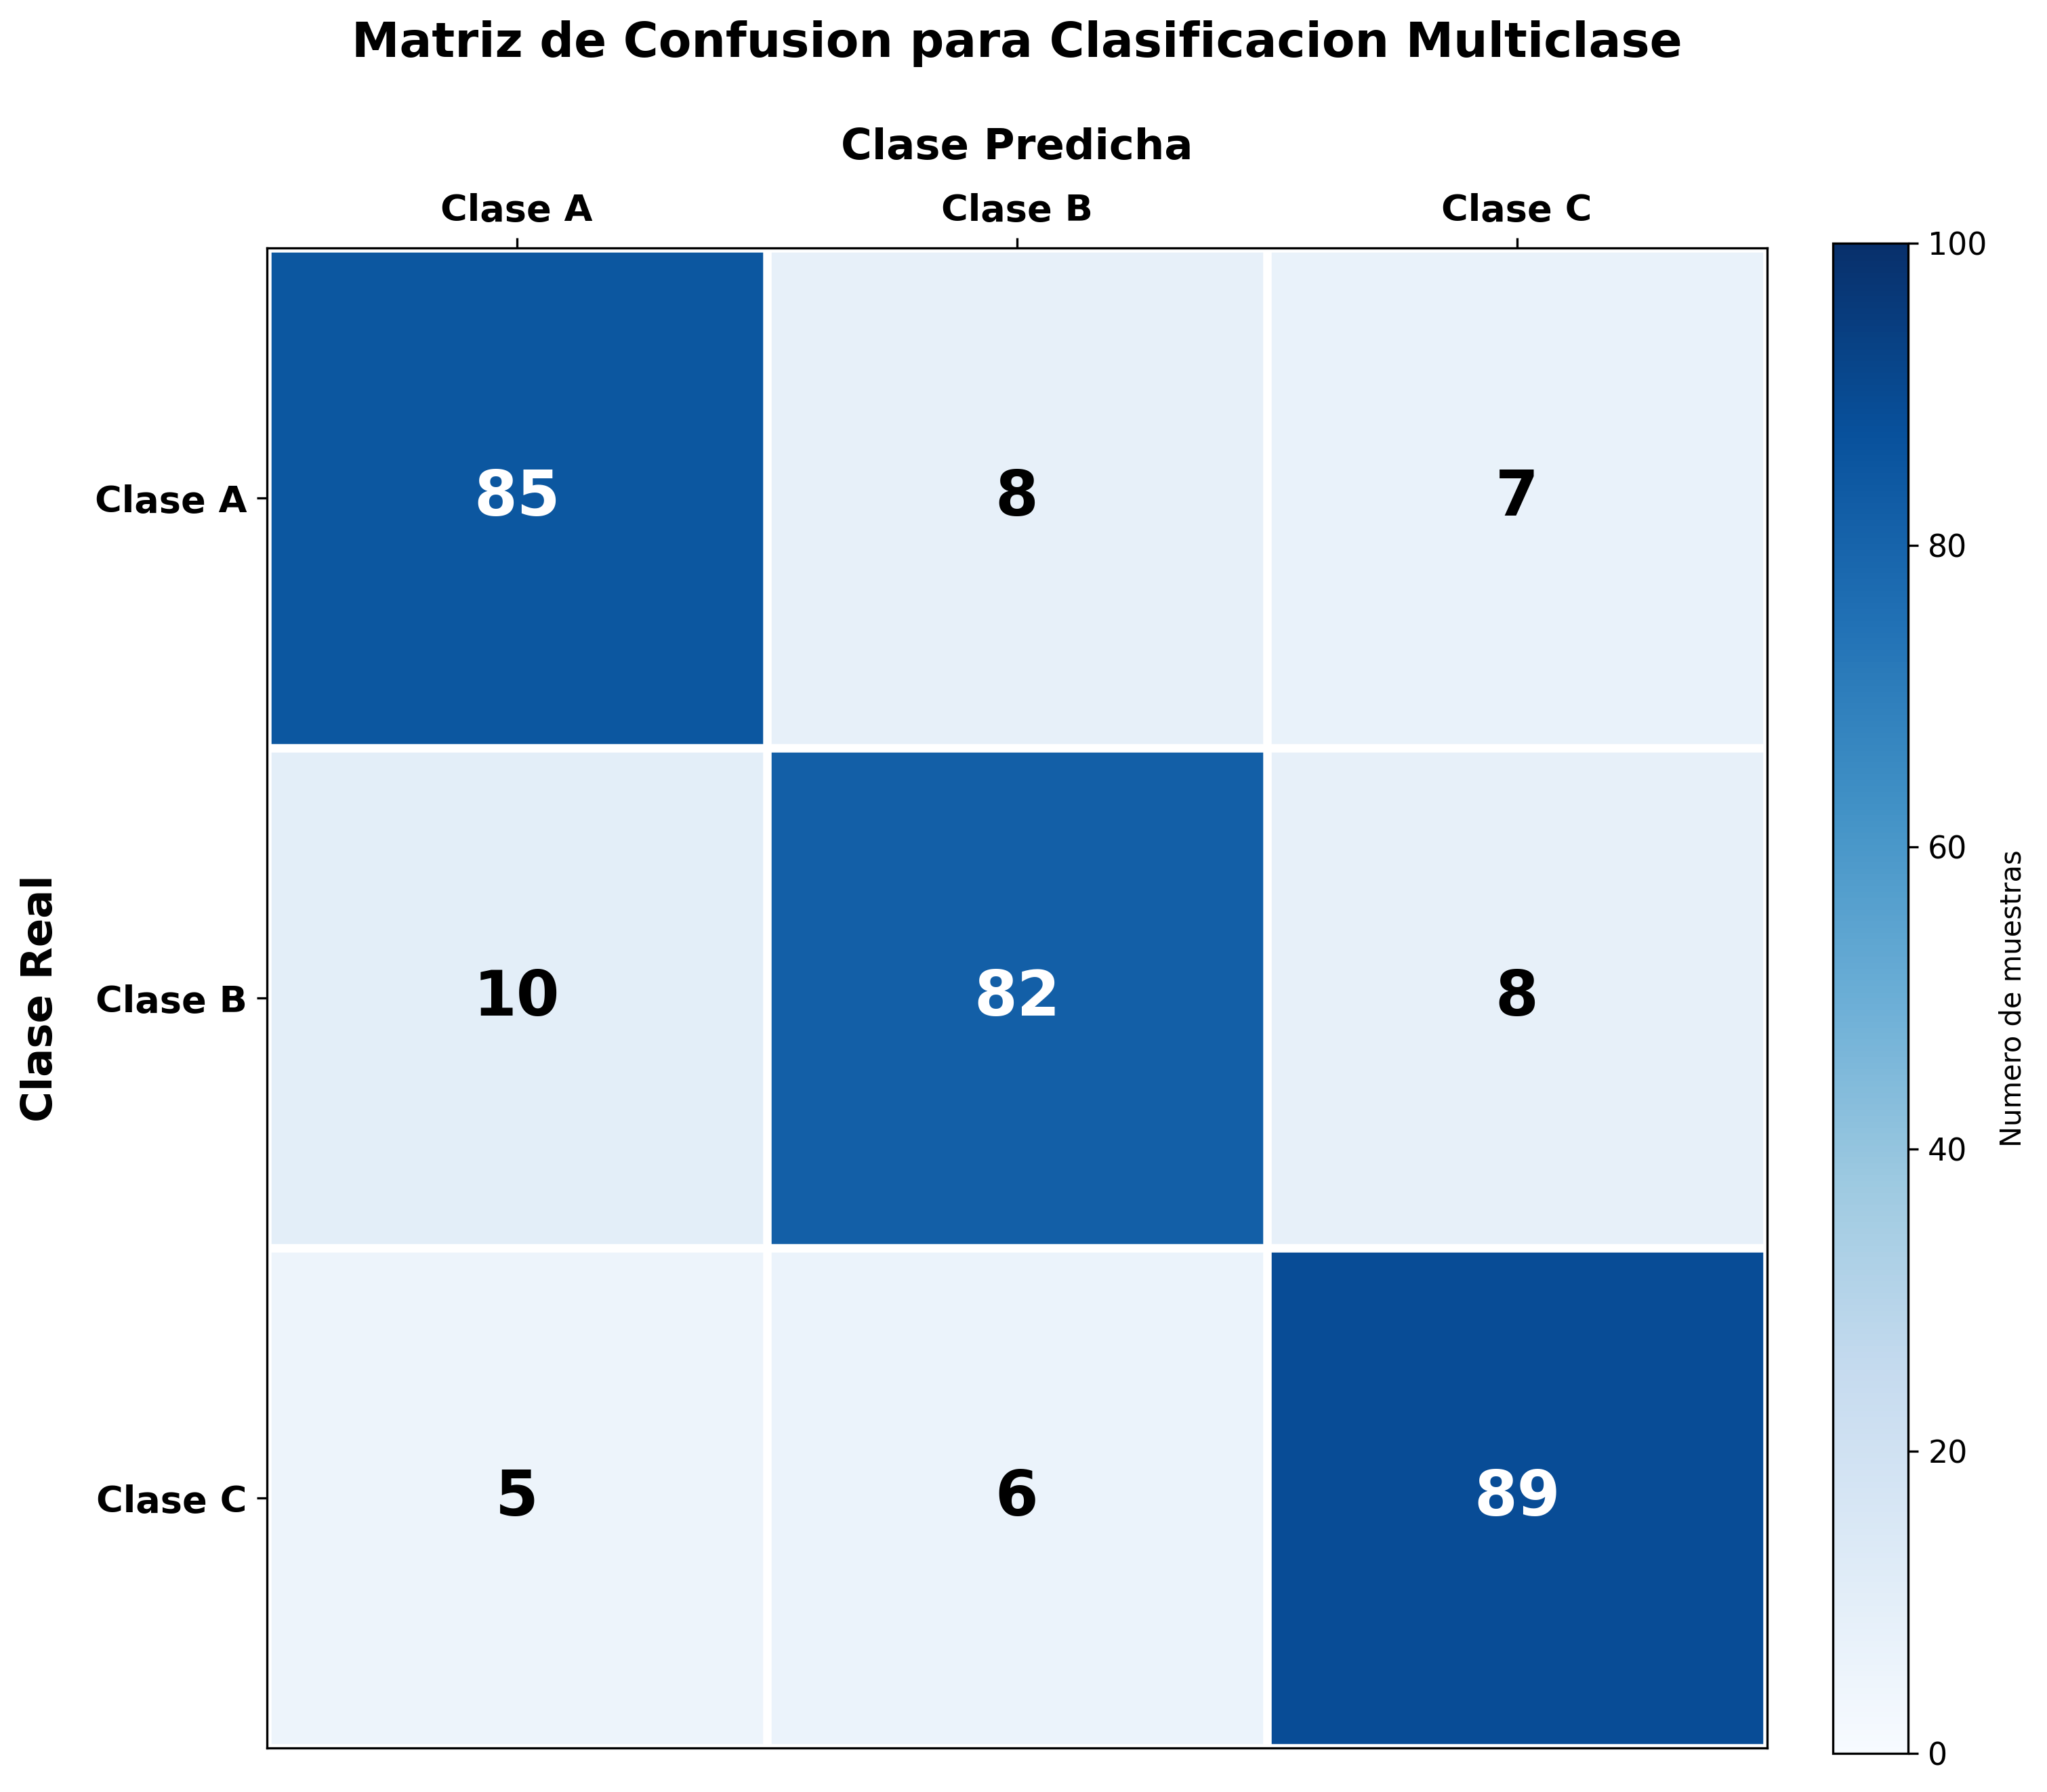
\includegraphics[width=0.65\textwidth]{imagenes/matriz_confusion_ejemplo.png}
\caption{Matriz de confusión para clasificación multiclase. Los elementos diagonales representan clasificaciones correctas, mientras que los elementos fuera de la diagonal indican errores de clasificación entre clases.}
\label{fig:matriz_confusion}
\end{figure}

\subsubsection{Exactitud, Precisión y Exhaustividad}

La \textbf{exactitud} mide la proporción global de predicciones correctas:

\begin{equation}
\text{Accuracy} = \frac{\text{TP} + \text{TN}}{\text{TP} + \text{TN} + \text{FP} + \text{FN}} = \frac{\sum_{i=1}^{C} M_{ii}}{N}
\end{equation}

Esta métrica es intuitiva y apropiada cuando todas las clases tienen igual importancia y están balanceadas. Sin embargo, resulta engañosa en datasets desbalanceados: un clasificador que siempre predice la clase mayoritaria puede alcanzar alta exactitud sin aprender patrones útiles. Por ejemplo, en un dataset con 95\% de negativos, predecir siempre negativo resulta en 95\% de exactitud sin detectar ningún positivo.

La \textbf{precisión} cuantifica la proporción de predicciones positivas que son correctas:

\begin{equation}
\text{Precision} = \frac{\text{TP}}{\text{TP} + \text{FP}}
\end{equation}

Esta métrica responde: de todas las instancias clasificadas como positivas, ¿qué fracción realmente lo era? La precisión es crucial cuando el costo de falsos positivos es alto, como en cosecha automatizada donde se debe evitar intentar cosechar elementos no deseados.

La \textbf{exhaustividad} (recall o sensitivity) mide la proporción de casos positivos reales que fueron correctamente identificados:

\begin{equation}
\text{Recall} = \frac{\text{TP}}{\text{TP} + \text{FN}}
\end{equation}

Esta métrica responde: de todas las instancias que realmente son positivas, ¿qué fracción detectó el modelo? El recall es fundamental cuando el costo de falsos negativos es alto, como en detección de productos maduros donde no se deben perder elementos listos para cosecha.

Existe un compromiso inherente entre precisión y recall: aumentar el umbral de decisión incrementa la precisión pero reduce el recall, y viceversa. Para problemas multiclase, estas métricas se calculan por clase mediante $\text{Precision}_i = M_{ii}/\sum_{j} M_{ji}$ y $\text{Recall}_i = M_{ii}/\sum_{j} M_{ij}$, pudiendo agregarse mediante promedio simple (macro-average) o ponderado por frecuencia de clase (weighted-average).

\subsubsection{Métricas para Validación de Calibración}

En sistemas que utilizan regresión para establecer transformaciones espaciales, como la calibración píxel-milímetro, se emplean métricas de error continuo. El \textbf{error cuadrático medio} (RMSE) cuantifica la magnitud típica de los errores:

\begin{equation}
\text{RMSE} = \sqrt{\frac{1}{N}\sum_{i=1}^{N}(y_i - \hat{y}_i)^2}
\end{equation}

donde $y_i$ son los valores verdaderos y $\hat{y}_i$ las predicciones del modelo. El RMSE penaliza fuertemente errores grandes debido a la elevación al cuadrado, resultando apropiado cuando se desea minimizar desviaciones extremas. El \textbf{coeficiente de determinación} $R^2$ complementa esta evaluación midiendo la proporción de varianza explicada por el modelo:

\begin{equation}
R^2 = 1 - \frac{\sum_{i=1}^{N}(y_i - \hat{y}_i)^2}{\sum_{i=1}^{N}(y_i - \bar{y})^2}
\end{equation}

donde $\bar{y}$ es la media de los valores observados. Valores de $R^2$ cercanos a 1 indican excelente ajuste lineal del modelo a los datos, mientras que valores cercanos a 0 indican que el modelo no captura la relación entre variables mejor que simplemente predecir el valor medio.

Para aplicaciones de agricultura de precisión, la selección de métricas debe alinearse con los objetivos operativos. En detección de cultivos para cosecha se prioriza alta exhaustividad (no perder productos maduros) manteniendo precisión aceptable (limitar intentos de cosecha erróneos). En calibración espacial se requiere bajo RMSE (típicamente <2mm) y alto $R^2$ (>0.99) para garantizar precisión en el posicionamiento del robot.
